\section*{Ethics and Law}
Notice in the last section there was the mention of enforcement in the discussion on bribery and corruption.  This issue begs a brief discussion of an important difference between law and ethics.  Law, or more precisely legal behavior, is behavior and conduct and actions that are in agreement with codified (written) standards in some legal documents by some appointed \footnote{The method of appointment is irrelevant, the legal body can be directly elected, appointed, or self-appointed, although the latter method might meet considerable resistance in the USA} 
legal body; those documents and the legal experts together determine what is law and whom should obey it.  The key points are that law is codified(written), interpreted by a legal body (the courts), the
documents and the legal body determines what is legal, and \textbf{may not apply to all}.

Figure   \ref{fig:ethics_and_law} presents a popular perception of ethical and legal behavior -- no doubt reinforced by the news media's coverage of congressional ethics.    There is probably some element truth to the dilemma proposed by the comic strip, but in business situations, such a dichotomy of behavior is probably rare.

\begin{figure}[ht!] %  figure placement: here, top, bottom, or page
   \centering
   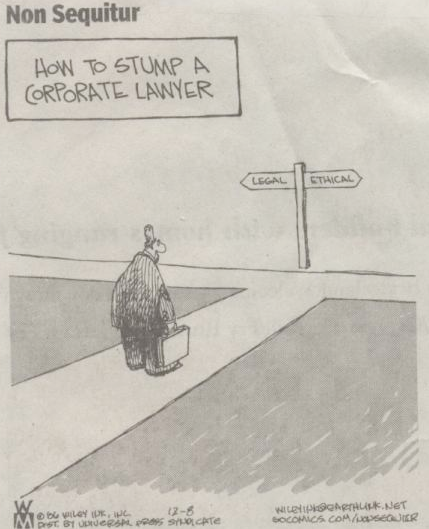
\includegraphics[width=5in]{./figures/ethics_and_law.pdf} 
   \caption{A popular view of ethics and law as it pertains to business; that is they are diametrically opposed.}
   \label{fig:ethics_and_law}
\end{figure}

Ethics, or more precisely ethical behavior, is behavior and conduct and actions that lead to outcomes that are socially acceptable (beneficial) and do not unduly impact individual rights.  In contrast to legal behavior, ethical behavior is defined by society, not necessarily written, exists independently of any ''experts,'' and applies to all members of society.  The distinction is subtle but important - things that are unethical are not necessarily illegal.  The converse is probably also true in some instances.  This brings us to the important part of the seminar, which are tools for making ethical choices.

\begin{figure}[ht!] %  figure placement: here, top, bottom, or page
   \centering
   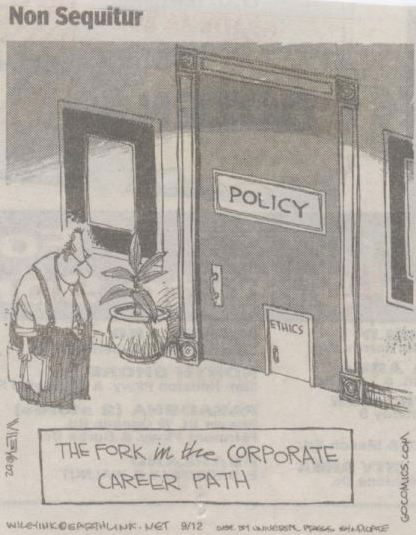
\includegraphics[width=5in]{./figures/ethics_or_business.pdf} 
   \caption{Another view of business principles (policy) and ethics; notice both doors go to the same place.}
   \label{fig:ethics_or_business}
\end{figure}

Figure  \ref{fig:ethics_or_business} is an alternate view of business and ethical behavior, and is probably a more meaningful allegory.  Both doors enter into the same place, the ethical door is smaller and requires far greater effort to squeeze through, while the policy door is huge.